\documentclass[aspectratio=169,10pt]{beamer}
\usepackage[english]{babel}
\usepackage[utf8]{inputenc}
\usepackage[T1]{fontenc}
\usepackage{lmodern,booktabs,tabularx,amsmath,tikz}
\usetikzlibrary{arrows.meta,positioning,fit,calc,shapes.geometric}
\usetheme{Madrid}
\definecolor{Ink}{HTML}{243748}
\definecolor{Muted}{HTML}{667B8B}
\definecolor{Accent}{HTML}{347E74}
\definecolor{AccentBlue}{HTML}{507DAD}
\definecolor{SoftMint}{HTML}{E6F4EE}
\definecolor{SoftLilac}{HTML}{F1EEF8}
\definecolor{Paper}{HTML}{FBFCFE}
\setbeamercolor{background canvas}{bg=Paper}
\setbeamercolor{normal text}{fg=Ink}
\setbeamercolor{structure}{fg=Accent}
\setbeamercolor{frametitle}{fg=Ink,bg=Paper}
\setbeamercolor{footline}{fg=Muted,bg=Paper}
\setbeamercolor{block title}{fg=Accent,bg=Paper}
\setbeamercolor{block body}{fg=Ink,bg=Paper}
\setbeamerfont{frametitle}{size=\large,series=\bfseries}
\setbeamertemplate{headline}{}
\setbeamertemplate{navigation symbols}{}
\setbeamersize{text margin left=.55cm,text margin right=.55cm}
\setbeamertemplate{frametitle}{\nointerlineskip\begin{beamercolorbox}[wd=\paperwidth,ht=.73cm,dp=.14cm,leftskip=.58cm]{frametitle}\usebeamerfont{frametitle}\insertframetitle\end{beamercolorbox}}
\setbeamertemplate{footline}{\begin{beamercolorbox}[wd=\paperwidth,ht=.31cm,dp=.14cm]{footline}\hspace{.55cm}\scriptsize\ifnum\value{framenumber}<20 Kareto Paper Review\hfill Main \insertframenumber/19\else Research backup\hfill B\number\numexpr\value{framenumber}-19\relax\fi\hspace{.55cm}\end{beamercolorbox}}
\newcommand{\src}[1]{\par\vspace{.03cm}{\tiny\color{Muted}#1}}
\newcommand{\take}[1]{\vspace{.05cm}\begin{beamercolorbox}[wd=\linewidth,sep=.07cm]{mintbox}\small\bfseries\color{Accent}#1\end{beamercolorbox}}
\newcommand{\tagline}[1]{{\small\color{Muted}#1\par}\vspace{.1cm}}
\newcommand{\jump}[2]{\hfill\hyperlink{#1}{\beamergotobutton{#2}}}
\newcommand{\back}[2]{\hfill\hyperlink{#1}{\beamerreturnbutton{#2}}}
\newcommand{\pic}[3]{\begin{center}\includegraphics[width=#2\linewidth,height=#3,keepaspectratio]{#1}\end{center}}
\newcommand{\concept}{\tiny\color{Muted}Conceptual illustration based on Kareto, Section 3.3.}
\newcommand{\proposal}{\tiny\color{Muted}Proposed research framework: not an evaluated result.}
\newcommand{\target}[1]{\hypertarget{#1}{}}
\begin{document}

% MAIN SLIDES (18)
\begin{frame}[t]
\vspace{.20cm}
{\large\bfseries Adaptive Multi-Objective Tiered Storage Configuration for KV Cache in LLM Service\par}
\vspace{.12cm}{\normalsize\color{Accent}Kareto | arXiv preprint | Workload-Aware KV Cache Storage Provisioning\par}
\vspace{.02cm}{\small\color{Muted}arXiv:2603.08739v1 | 25 February 2026\par}
\vspace{.06cm}{\small Xianzhe Zheng et al. | Zhejiang University and Alibaba Group\par}
\vspace{.12cm}
\begin{columns}[T,onlytextwidth]
\begin{column}{.35\textwidth}\centering
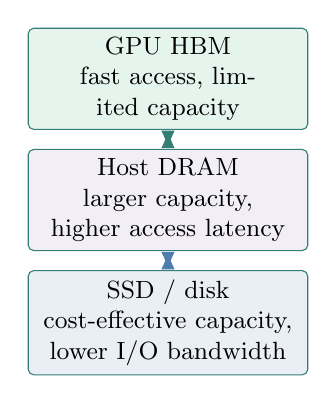
\begin{tikzpicture}[>=Latex,node distance=.24cm,box/.style={draw=Accent,rounded corners=2pt,text width=3.25cm,minimum width=3.55cm,minimum height=.60cm,align=center,font=\small}]
\node[box,fill=SoftMint](h){GPU HBM\\fast access, limited capacity};
\node[box,fill=SoftLilac,below=of h](d){Host DRAM\\larger capacity, higher access latency};
\node[box,fill=AccentBlue!12,below=of d](s){SSD / disk\\cost-effective capacity, lower I/O bandwidth};
\draw[<->,thick,Accent](h)--(d);\draw[<->,thick,AccentBlue](d)--(s);
\end{tikzpicture}
\end{column}
\begin{column}{.53\textwidth}
\begin{tabularx}{\linewidth}{>{\bfseries\color{Accent}}p{2.35cm}X}
Limited HBM & Long contexts and concurrent requests increase KV-cache capacity requirements.\\[.11cm]
Static provisioning & Predefined capacities can over-provision or under-provision storage.\\[.11cm]
Workload diversity & Reuse patterns and request density change the value of each tier.
\end{tabularx}
\end{column}
\end{columns}
{\small\bfseries\color{Accent}Kareto adapts storage to workload and service objectives.\par}
\src{Source: Kareto v1, Abstract and §§1–2, pp. 1–2. Preprint; no venue claim.}
\end{frame}

\begin{frame}[t]{Workload-Dependent KV Cache Reuse}
\target{main-reuse}\tagline{Reuse-hit concentration differs sharply across workloads}
\begin{columns}[T,onlytextwidth]
\begin{column}{.67\textwidth}\pic{Kareto-Adaptive-Tiered-KV-Cache-2026/Without-Caption/Kareto_Fig02.png}{1.0}{3.0cm}\end{column}
\begin{column}{.31\textwidth}
{\Large\bfseries 31.95\%\par}{\small of Trace A KV blocks account for 90\% of reuse hits.\par}\vspace{.3cm}
{\Large\bfseries 0.67\%\par}{\small of Trace B KV blocks account for 90\% of reuse hits.\par}\vspace{.25cm}
\small Trace A: interactive chatbot.\\Trace B: programmatic API, with concentrated shared-prefix reuse.\\[.12cm]\textbf{These are reuse-hit concentration values, not overall cache hit rates.}
\end{column}
\end{columns}
{\small\bfseries\color{Accent}The effective KV-cache working set depends on workload-specific reuse patterns.\par}
\src{Source: Kareto v1, Section 3.1, Figure 2, p. 3.}\jump{backup-lifetime}{TTL detail}
\end{frame}

\begin{frame}[t]{Cache Capacity Saturation and Diminishing Returns}
\target{main-saturation}\tagline{Capacity adds reuse, but marginal gains fall after the working set is covered}
\begin{columns}[T,onlytextwidth]
\begin{column}{.62\textwidth}\pic{Kareto-Adaptive-Tiered-KV-Cache-2026/Without-Caption/Kareto_Fig03.png}{1.0}{4.6cm}\end{column}
\begin{column}{.35\textwidth}
\begin{block}{Reported example}\small Increasing capacity from 250 GB to 1,000 GB yields about 21\% higher reuse ratio.\\[.18cm]Increasing from 1,000 GB to 2,000 GB yields less than 7\% additional improvement.\end{block}
\small The effective cache size is a workload property. Beyond saturation, storage cost can keep rising while reuse gains taper.
\end{column}
\end{columns}
\take{Capacity planning must account for diminishing returns, not capacity alone.}
\src{Source: Kareto v1, Section 3.1.2, Figure 3, p. 4.}\jump{backup-lifetime}{TTL and lifetime}
\end{frame}

\begin{frame}[t]{Workload Density Changes the Value of SSD Prefetching}
\target{main-density}\tagline{Kareto uses existing queue time as a prefetch window; it does not add queueing deliberately}
\begin{columns}[T,onlytextwidth]
\begin{column}{.48\textwidth}\centering{\large\bfseries Compute-abundant / low density\par}\vspace{.2cm}
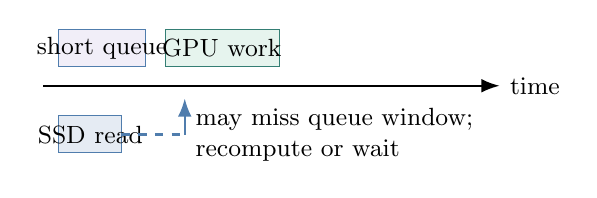
\begin{tikzpicture}[x=1cm,y=1cm,>=Latex,font=\small]
\draw[->,thick](0,0)--(5.8,0) node[right]{time};\draw[fill=SoftLilac,draw=AccentBlue](.2,.25) rectangle (1.3,.72);\node at (.75,.48){short queue};
\draw[fill=SoftMint,draw=Accent](1.55,.25) rectangle (3.0,.72);\node at (2.27,.48){GPU work};
\draw[fill=AccentBlue!15,draw=AccentBlue](.2,-.85) rectangle (1.0,-.38);\node at (.6,-.62){SSD read};\draw[dashed,thick,AccentBlue](1,-.62)--(1.8,-.62);\draw[->,thick,AccentBlue](1.8,-.62)--(1.8,-.16);\node[align=left] at (3.7,-.62){may miss queue window;\\recompute or wait};
\end{tikzpicture}
\small Short queues limit prefetch opportunity; disk reload can be slower than recomputation.
\end{column}
\begin{column}{.48\textwidth}\centering{\large\bfseries Compute-constrained / high density\par}\vspace{.2cm}
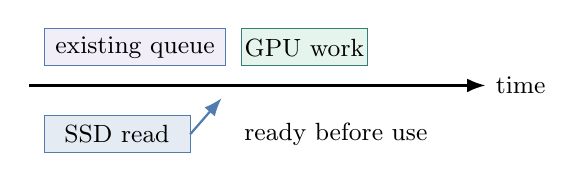
\begin{tikzpicture}[x=1cm,y=1cm,>=Latex,font=\small]
\draw[->,thick](0,0)--(5.8,0) node[right]{time};\draw[fill=SoftLilac,draw=AccentBlue](.2,.25) rectangle (2.5,.72);\node at (1.35,.48){existing queue};
\draw[fill=SoftMint,draw=Accent](2.7,.25) rectangle (4.3,.72);\node at (3.5,.48){GPU work};
\draw[fill=AccentBlue!15,draw=AccentBlue](.2,-.85) rectangle (2.05,-.38);\node at (1.12,-.62){SSD read};\draw[->,thick,AccentBlue](2.05,-.62)--(2.45,-.16);\node at (3.9,-.62){ready before use};
\end{tikzpicture}
\small Longer existing queues can hide more disk I/O and enable cache reuse.
\end{column}
\end{columns}
\vspace{-.02cm}{\concept\par}
\take{SSD caching helps when its data becomes ready before dependent GPU computation.}
\src{Source: Kareto v1, Section 3.3, observations 1–4, pp. 5–6.}\jump{backup-density}{Figures 5–6}
\end{frame}

\begin{frame}[t]{Density Changes Reuse, Throughput, and TTFT}
\target{main-density-data}\tagline{Figure 5 compares capacity effects in compute-bound and compute-abundant settings}
\pic{Kareto-Adaptive-Tiered-KV-Cache-2026/Without-Caption/Kareto_Fig05.png}{.98}{3.9cm}
\begin{columns}[T,onlytextwidth]\begin{column}{.48\textwidth}\small\textbf{Compute-bound / 1 instance} More capacity reduces redundant prefill; throughput can rise with reuse.\end{column}\begin{column}{.48\textwidth}\small\textbf{Compute-abundant / 4 instances} Throughput approaches request arrivals; capacity chiefly affects latency and reuse.\end{column}\end{columns}
\take{The same capacity increase has different value as workload density changes.}
\src{Original Figure 5, Kareto v1, Section 3.3, p. 5.}\jump{backup-density}{Figure 5 detail}\jump{backup-density-full}{Figure 6 detail}
\end{frame}

\begin{frame}[t]{Kareto Optimizes Throughput, Latency, and Economic Cost}
\target{main-objectives}\tagline{The objectives define a Pareto set, not one universal optimum}
\begin{columns}[T,onlytextwidth]
\begin{column}{.47\textwidth}
\begin{block}{Problem formulation}\large\[
\min_{\mathbf{x}\in\mathcal{X}}\left(\mathbb{E}[L(\mathbf{x})],-\mathbb{E}[T(\mathbf{x})],C(\mathbf{x})\right)
\]\end{block}
\small Decision space includes workload, compute, storage medium, and management policy. Evaluated planner sweeps DRAM capacity and TTL while holding the medium fixed to ESSD PL1.
\end{column}
\begin{column}{.50\textwidth}\pic{Kareto-Adaptive-Tiered-KV-Cache-2026/Without-Caption/Kareto_Fig08.png}{1.0}{3.9cm}\small Original two-instance comparison: pure DRAM, pure disk, and hybrid with 256 GB DRAM plus varying disk. Hybrid trades cost against latency while maintaining throughput.\end{column}
\end{columns}
\take{Different service objectives favor different non-dominated storage configurations.}
\src{Source: Kareto v1, Section 3.1, Eqs. 1–2 and Figure 8, pp. 3–4, 7. Cost is economic expenditure, not energy.}\jump{backup-bandwidth}{Bandwidth sensitivity}
\end{frame}

\begin{frame}[t]{Kareto Uses an End-to-End Discrete-Event Simulator}
\target{main-simulator}\tagline{The authors develop their own trace-driven simulator; it is not LLMServingSim}
\pic{Kareto-Adaptive-Tiered-KV-Cache-2026/Without-Caption/Kareto_Fig04.png}{.40}{2.55cm}
\begin{center}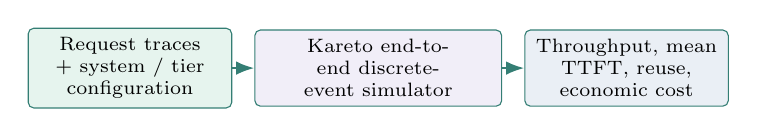
\begin{tikzpicture}[>=Latex,node distance=.28cm,box/.style={draw=Accent,rounded corners=2pt,fill=SoftMint,minimum height=.54cm,text width=2.35cm,align=center,font=\scriptsize}]
\node[box](a){Request traces + system / tier configuration};\node[box,right=of a,fill=SoftLilac,text width=2.9cm](b){Kareto end-to-end discrete-event simulator};\node[box,right=of b,fill=AccentBlue!12](c){Throughput, mean TTFT, reuse, economic cost};\draw[->,thick,Accent](a)--(b);\draw[->,thick,Accent](b)--(c);
\end{tikzpicture}\end{center}
\take{The simulator captures interactions among inference execution, KV-cache management, and storage tiers.}
\src{Figure 4 and Section 3.2, p. 4. Figure 4 is displayed with original panels and labels.}\jump{backup-simulator}{Architecture detail}
\end{frame}

\begin{frame}[t]{Empirical GPU Profiling Feeds Execution-Time Models}
\target{main-profiling}\tagline{Kernel execution time is profiled on target GPUs and interpolated across lengths}
\begin{columns}[T,onlytextwidth]
\begin{column}{.51\textwidth}\centering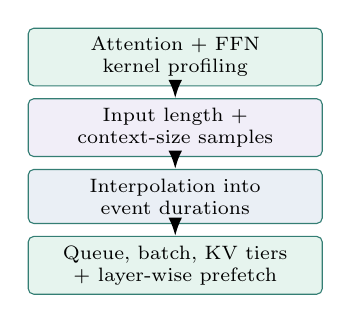
\begin{tikzpicture}[>=Latex,node distance=.15cm,box/.style={draw=Accent,rounded corners=2pt,minimum height=.52cm,text width=3.5cm,align=center,font=\scriptsize}]
\node[box,fill=SoftMint](a){Attention + FFN kernel profiling};\node[box,fill=SoftLilac,below=of a](b){Input length + context-size samples};\node[box,fill=AccentBlue!12,below=of b](c){Interpolation into event durations};\node[box,fill=SoftMint,below=of c](d){Queue, batch, KV tiers + layer-wise prefetch};\draw[->,thick](a)--(b);\draw[->,thick](b)--(c);\draw[->,thick](c)--(d);\end{tikzpicture}\end{column}
\begin{column}{.45\textwidth}\small\textbf{Simulator models}\\Request arrivals / queueing; inference and batching; radix-tree prefix reuse; hierarchical placement, eviction, storage I/O, and prefetch stalls.\\[.15cm]\textbf{Outputs}\\Throughput, mean TTFT, cache reuse, and economic cost.\end{column}
\end{columns}
\vspace{.12cm}\small Kareto's GPU profiling models execution time. It does not report the four phase-specific power models proposed later here.
\take{The published simulator supports performance exploration; energy fidelity remains a separate research task.}
\src{Source: Kareto v1, Section 3.2 and Figure 4, p. 4. Profiling-table structure is not fully disclosed.}\jump{backup-simulator}{Simulator details}
\end{frame}

\begin{frame}[t]{Adaptive Pareto Search Refines High-Impact Regions}
\target{main-search}\tagline{Coarse sampling identifies where further simulation is useful}
\begin{columns}[T,onlytextwidth]
\begin{column}{.56\textwidth}\centering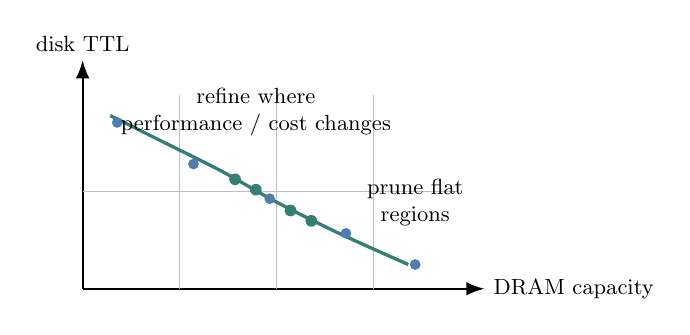
\begin{tikzpicture}[>=Latex,scale=.88,transform shape,font=\small]
\draw[->,thick](0,0)--(5.8,0) node[right]{DRAM capacity};\draw[->,thick](0,0)--(0,3.3) node[above]{disk TTL};
\draw[gray!50](1.4,0)--(1.4,2.8);\draw[gray!50](2.8,0)--(2.8,2.8);\draw[gray!50](4.2,0)--(4.2,2.8);\draw[gray!50](0,1.4)--(5.4,1.4);
\draw[Accent,very thick] plot[smooth] coordinates{(.4,2.5)(1.2,2.1)(2.0,1.7)(2.8,1.25)(3.7,.8)(4.7,.35)};
\foreach \x/\y in {.5/2.4,1.6/1.8,2.7/1.3,3.8/.8,4.8/.35}{\fill[AccentBlue] (\x,\y) circle (2.2pt);}
\foreach \x/\y in {2.2/1.58,2.5/1.43,3.0/1.13,3.3/.98}{\fill[Accent] (\x,\y) circle (2.4pt);}
\node[align=center] at (2.5,2.55){refine where\\performance / cost changes};\node[align=center] at (4.8,1.25){prune flat\\regions};
\end{tikzpicture}\par{\concept}\end{column}
\begin{column}{.40\textwidth}\begin{enumerate}\small\item Start from a coarse DRAM–TTL grid.\item Expand while marginal gains justify more capacity.\item Add points in high-variation regions.\item Pareto-filter evaluated configurations.\end{enumerate}\small The reported ablation uses fewer search evaluations than grid search with similar hypervolume. It does not establish a mathematical global optimum.\end{column}
\end{columns}
\take{Adaptive exploration spends simulations where configuration changes matter.}
\src{Source: Kareto v1, Section 4.2, Algorithm 1; Section 5.3.1, Figure 13.}\jump{backup-search}{Search ablation}
\end{frame}

\begin{frame}[t]{Group TTL Allocates Disk Retention by Reuse Pattern}
\target{main-groupttl}\tagline{TTL means time-to-live: the duration a KV block remains in the disk tier}
\begin{columns}[T,onlytextwidth]
\begin{column}{.52\textwidth}\pic{Kareto-Adaptive-Tiered-KV-Cache-2026/Without-Caption/Kareto_Fig10.png}{.98}{3.65cm}\small A few prefix-tree subtrees account for most reuse events.\end{column}
\begin{column}{.45\textwidth}\centering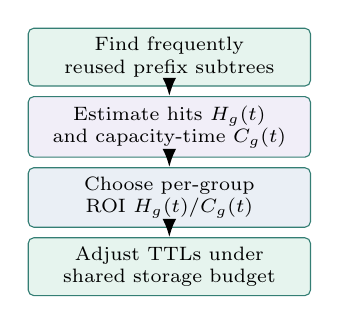
\begin{tikzpicture}[>=Latex,node distance=.12cm,box/.style={draw=Accent,rounded corners=2pt,fill=SoftMint,text width=3.35cm,minimum height=.40cm,align=center,font=\scriptsize}]
\node[box](a){Find frequently reused prefix subtrees};\node[box,below=of a,fill=SoftLilac](b){Estimate hits $H_g(t)$ and capacity-time $C_g(t)$};\node[box,below=of b,fill=AccentBlue!12](c){Choose per-group ROI $H_g(t)/C_g(t)$};\node[box,below=of c](d){Adjust TTLs under shared storage budget};\draw[->,thick](a)--(b);\draw[->,thick](b)--(c);\draw[->,thick](c)--(d);\end{tikzpicture}\end{column}
\end{columns}
\scriptsize ROI means hits per capacity-time, not profit or energy saved. TTL applies to disk retention.\par\vspace{.04cm}\take{Workload-aware TTL complements capacity exploration.}
\src{Source: Kareto v1, Sections 4.1–4.3, Figures 9–11, Algorithms 1–2.}\jump{backup-groupttl}{Reuse groups}\jump{backup-groupttl-formula}{ROI allocation}
\end{frame}

\begin{frame}[t]{Evaluation Uses Three Trace Types and Two Cluster Scales}
\target{main-setup}\tagline{The paper evaluates a Qwen3-480B / SGLang serving setup with ESSD PL1}
\begin{columns}[T,onlytextwidth]
\begin{column}{.50\textwidth}\begin{tabularx}{\linewidth}{lX}\toprule\textbf{Trace}&\textbf{Workload}\\\midrule
A&Interactive chatbot; open-source dataset derived\\
B&Programmatic API; shared prompts, open-source dataset derived\\
C&Synthetic agent workload reflecting internal request characteristics\\\bottomrule\end{tabularx}\par\vspace{.12cm}\small Each trace spans two hours and contains 40k–170k requests. Trace C is synthetic; the traces are not all production traces.\end{column}
\begin{column}{.47\textwidth}\begin{block}{System and scenarios}\small Model: Qwen3-480B\\Serving engine: SGLang\\Storage: Alibaba Cloud ESSD PL1\\1 instance: compute-constrained\\4 instances: compute-abundant\\Baseline: fixed 1,024 GB DRAM\end{block}\scriptsize Instance counts refer to cloud compute instances, not GPU counts. Exact accelerator / parallelism configuration for the emulated evaluation is not confirmed in the paper.\end{column}
\end{columns}
\take{Workload provenance and compute scale shape how the reported outcomes should be read.}
\src{Source: Kareto v1, Sections 3.3 and 5.1–5.2, pp. 5, 9–10.}\jump{backup-bandwidth}{Storage sensitivity}
\end{frame}

\begin{frame}[t]{Simulator Fidelity Is Validated on Three Storage Configurations}
\target{main-validation}\tagline{Real-system comparisons isolate GPU-only, GPU + host DRAM, and GPU + disk}
\pic{Kareto-Adaptive-Tiered-KV-Cache-2026/Without-Caption/Kareto_Fig17.png}{.96}{3.0cm}
\begin{columns}[T,onlytextwidth]\begin{column}{.32\textwidth}\centering{\Large\bfseries 19.2\%}\par\small maximum mean-TTFT deviation\end{column}\begin{column}{.32\textwidth}\centering{\Large\bfseries 6.5\%}\par\small maximum throughput deviation\end{column}\begin{column}{.32\textwidth}\centering{\Large\bfseries 2.0\%}\par\small maximum cache-hit-rate deviation\end{column}\end{columns}
\small GPU-only means the KV-cache tier is GPU memory; it does not mean CPU/host resources are absent. These are maximum deviations for the tested metrics and configurations, not average errors or validation of power, energy, carbon, or TPOT.
\take{Validation supports simulation-driven exploration within the evaluated configurations.}
\src{Source: Kareto v1, Section 5.4, Figure 17 (HTML calls this Figure 19), pp. 13–14.}\jump{backup-validation}{Validation details}
\end{frame}

\begin{frame}[t]{Adaptive Provisioning Improves Distinct Objectives}
\target{main-gains}\tagline{Compared with fixed 1,024 GB DRAM; maxima come from separate objective-specific choices}
\pic{Kareto-Adaptive-Tiered-KV-Cache-2026/Without-Caption/Kareto_Fig12.png}{.85}{3.3cm}
\begin{columns}[T,onlytextwidth]\begin{column}{.32\textwidth}\centering{\Large\bfseries +9.3\%}\par\small maximum throughput\end{column}\begin{column}{.32\textwidth}\centering{\Large\bfseries $-58.3\%$}\par\small maximum mean TTFT\end{column}\begin{column}{.32\textwidth}\centering{\Large\bfseries $-20.2\%$}\par\small maximum economic cost\end{column}\end{columns}
\small Under 1 instance, storage can reduce redundant prefill work; under 4 instances, throughput is arrival-limited and right-sizing mainly reduces cost. Search and group TTL benefits vary by workload and density.
\take{These separate maxima are not simultaneous gains from one configuration.}
\src{Source: Kareto v1, Sections 5.2–5.3, Figure 12, pp. 10–14. Cost means economic expenditure.}\jump{backup-ablation}{Ablations}
\end{frame}

\begin{frame}[t]{Kareto and GreenCache Address Complementary Decisions}
\target{main-priorwork}\tagline{Prior work contributes complementary methods and objectives}
\begin{columns}[T,onlytextwidth]
\begin{column}{.48\textwidth}\begin{block}{Kareto | arXiv:2603.08739v1}\small Multi-tier KV configuration; workload-aware reuse; adaptive capacity and disk group TTL; end-to-end performance simulation.\par\smallskip\textbf{Objectives:} throughput, mean TTFT, economic cost.\par\textbf{Boundary:} no explicit energy or carbon optimization.\end{block}\end{column}
\begin{column}{.48\textwidth}\begin{block}{GreenCache | arXiv:2505.23970v3}\small Carbon-aware cache sizing and Least Carbon Savings replacement; operational and embodied carbon; TTFT / TPOT constraints.\par\smallskip\textbf{Power inputs:} CPU/GPU measured; DRAM/SSD use typical specification values.\par\textbf{Boundary:} storage energy not activity-measured.\end{block}\end{column}
\end{columns}
\take{The papers address complementary decisions with different objectives.}
\src{Sources: Kareto v1 Sections 3–5; GreenCache Sections 3, 5–6.}\jump{backup-accounting}{Accounting boundaries}
\end{frame}

\begin{frame}[t]{Energy-Aware Multi-Tier Cache Management Is a Gap to Validate}
\target{main-hypothesis}\tagline{Proposed direction: lower energy and carbon while meeting service constraints}
\begin{columns}[T,onlytextwidth]
\begin{column}{.48\textwidth}\begin{block}{Research hypotheses}\small Performance-optimal and cost-optimal configurations may differ from energy-optimal configurations.\par\smallskip A higher cache hit rate may not always reduce total system energy.\end{block}\begin{block}{Stage 1 objective}\small Minimize system energy subject to TTFT and TPOT SLOs, required goodput, memory capacity, and applicable power budget.\end{block}\end{column}
\begin{column}{.48\textwidth}\begin{block}{Potential gap to validate}\small Jointly model cache retention, tier placement, movement, and recomputation with measured component energy. Then consider operational and embodied carbon under declared workload, SLO, and lifecycle boundaries.\end{block}\begin{block}{Novelty boundary}\small This is a candidate gap, not a claim that no prior work exists. GreenCache already performs carbon-aware sizing and replacement.\end{block}\end{column}
\end{columns}
\take{Test these hypotheses under equal workload and SLO constraints.}
\src{Proposed research direction informed by Kareto v1 and GreenCache v3.}\jump{backup-break-even}{Break-even model}\jump{backup-accounting}{Accounting}
\end{frame}



\begin{frame}[t]{Energy-Aware Cache Decisions Must Respect Data Availability}
\target{main-decision}\tagline{Proposed decision path for a request under performance, capacity, and energy constraints}
\centering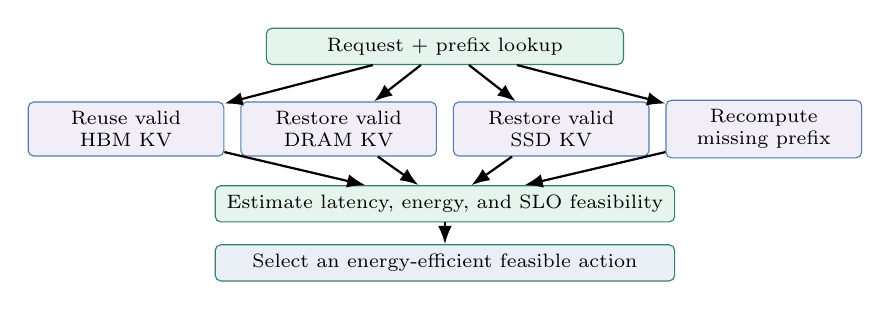
\begin{tikzpicture}[>=Latex,font=\scriptsize,box/.style={draw=Accent,rounded corners=2pt,fill=SoftMint,text width=4.3cm,minimum height=.46cm,align=center},act/.style={draw=AccentBlue,rounded corners=2pt,fill=SoftLilac,text width=2.25cm,minimum height=.58cm,align=center}]
\node[box] (r) at (5.5,0) {Request + prefix lookup};
\node[act] (h) at (1.45,-1.05) {Reuse valid HBM KV};
\node[act] (d) at (4.15,-1.05) {Restore valid DRAM KV};
\node[act] (s) at (6.85,-1.05) {Restore valid SSD KV};
\node[act] (c) at (9.55,-1.05) {Recompute missing prefix};
\node[box,text width=5.6cm] (e) at (5.5,-2.0) {Estimate latency, energy, and SLO feasibility};
\node[box,text width=5.6cm,fill=AccentBlue!12] (o) at (5.5,-2.75) {Select an energy-efficient feasible action};
\draw[->,thick](r)--(h);\draw[->,thick](r)--(d);\draw[->,thick](r)--(s);\draw[->,thick](r)--(c);\draw[->,thick](h)--(e);\draw[->,thick](d)--(e);\draw[->,thick](s)--(e);\draw[->,thick](c)--(e);\draw[->,thick](e)--(o);
\end{tikzpicture}\\{\proposal}
\small Restore is feasible only when requested KV data exists and is valid in that tier. Recomputation includes Attention and FFN across Transformer layers.
\take{The proposed policy considers retention, placement, transfers, and recomputation under SLOs.}
\src{Proposed research direction; not a Kareto or GreenCache evaluated result.}\jump{backup-break-even}{Energy model}
\end{frame}

\begin{frame}[t]{GPU Models Should Separate Prefill and Decode Operations}
\target{main-phase-model}\tagline{First-stage proposal: fit latency, power, and energy for four operation categories}
\begin{center}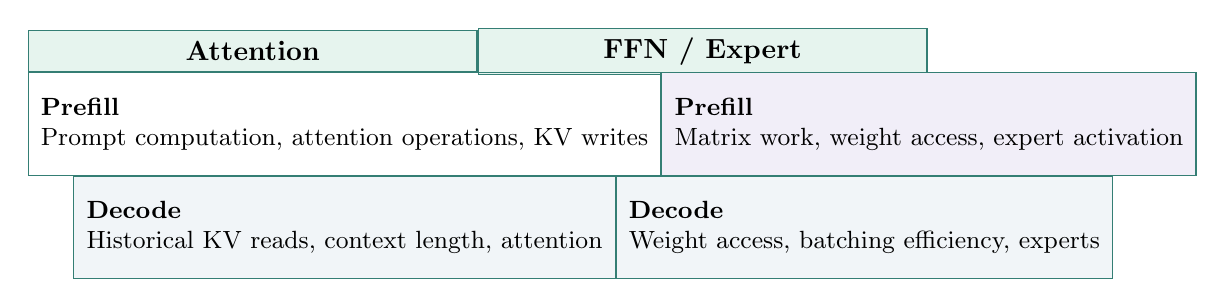
\begin{tikzpicture}[font=\small,cell/.style={draw=Accent,minimum width=5.7cm,minimum height=1.30cm,align=left,inner sep=.16cm},head/.style={fill=SoftMint,draw=Accent,minimum width=5.7cm,minimum height=.52cm,align=center,font=\bfseries}]
\node[head](h1){Attention};\node[head,right=0pt of h1](h2){FFN / Expert};
\node[cell,below=0pt of h1,anchor=north west] (p1) at ([yshift=0pt]h1.south west) {\textbf{Prefill}\\Prompt computation, attention operations, KV writes};
\node[cell,right=0pt of p1,fill=SoftLilac] (p2) {\textbf{Prefill}\\Matrix work, weight access, expert activation};
\node[cell,below=0pt of p1,fill=AccentBlue!8] (d1) {\textbf{Decode}\\Historical KV reads, context length, attention};
\node[cell,right=0pt of d1,fill=AccentBlue!8] (d2) {\textbf{Decode}\\Weight access, batching efficiency, experts};
\end{tikzpicture}\end{center}
\begin{columns}[T,onlytextwidth]\begin{column}{.48\textwidth}\small\textbf{Model outputs:} latency (ms), power (W), energy (J).\\\textbf{Parameters:} GPU, batch, new tokens, prefix/context length, model, precision, traffic, frequency, expert activation.\end{column}\begin{column}{.48\textwidth}\small Begin with dense Attention and FFN; model MoE expert operations later. Calibrate against measurements. No Attention/Expert disaggregation is assumed.\end{column}\end{columns}
\take{Phase- and operation-aware model fidelity must be measured, not assumed from detail.}
\src{Proposed research framework: not an evaluated result.}\jump{backup-accounting}{Energy accounting}
\end{frame}

\begin{frame}[t]{System Energy Requires Consistent Component Accounting}
\target{main-energy}\tagline{Count measured system power over time; account for shared work and overlapping activity}
\begin{columns}[T,onlytextwidth]
\begin{column}{.48\textwidth}\begin{block}{Proposed accounting boundary}\small GPU board and HBM accesses; CPU; host DRAM idle/read/write; SSD idle/read/write; PCIe and relevant interconnect; server baseline; shared batch work; prefetch and I/O contention.\end{block}
\small\[
\begin{aligned}
E_{IT}&=\int P_{IT}(t)\,dt\\
C_{op}&=\sum_t E_{IT,t}\cdot PUE_t\cdot CI_t\\
C_{total}&=C_{op}+C_{emb,alloc}
\end{aligned}
\]
\end{column}
\begin{column}{.48\textwidth}\small\textbf{Avoid accounting errors}\\Do not add HBM energy on top of a GPU-board measurement that already includes it.\\Do not add isolated per-request estimates to shared batch energy.\\Account for concurrent work and overlap. Apply PUE once.\\Treat embodied carbon as lifecycle allocation; eviction does not undo manufacturing emissions.\\At fixed CI and PUE, energy and operational-carbon rankings match. Occupancy reduction may not reduce physical idle power.\end{column}
\end{columns}
\take{Energy and carbon rankings depend on a validated boundary and consistent allocation.}
\src{Proposed research methodology. GreenCache distinguishes operational and embodied carbon.}\jump{backup-accounting}{Full boundaries}
\end{frame}

\begin{frame}[t]{A Validated Energy Model Can Guide SLO-Constrained Optimization}
\target{main-plan}\tagline{Proposed implementation sequence; LLMServingSim 2.0 remains a candidate foundation}
\begin{columns}[T,onlytextwidth]
\begin{column}{.55\textwidth}\centering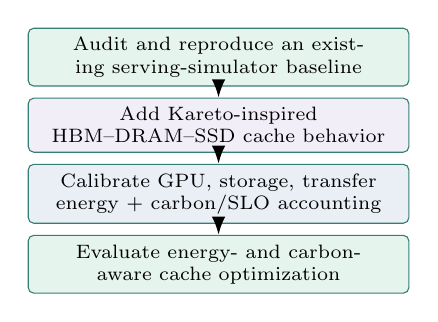
\begin{tikzpicture}[>=Latex,node distance=.14cm,font=\scriptsize,box/.style={draw=Accent,rounded corners=2pt,fill=SoftMint,text width=4.6cm,minimum height=.40cm,align=center}]
\node[box](a){Audit and reproduce an existing serving-simulator baseline};\node[box,below=of a,fill=SoftLilac](b){Add Kareto-inspired HBM–DRAM–SSD cache behavior};\node[box,below=of b,fill=AccentBlue!12](c){Calibrate GPU, storage, transfer energy + carbon/SLO accounting};\node[box,below=of c,fill=SoftMint](d){Evaluate energy- and carbon-aware cache optimization};
\draw[->,thick](a)--(b);\draw[->,thick](b)--(c);\draw[->,thick](c)--(d);
\end{tikzpicture}\\{\proposal}\end{column}
\begin{column}{.42\textwidth}\scriptsize\textbf{Next steps}\par 1. Audit simulators and power models.\par 2. Reproduce a baseline.\par 3. Profile GPU operations.\par 4. Calibrate storage / transfer energy.\par 5. Compare restore and recompute.\par 6. Test equal workload and SLOs.\par 7. Design policies after gap validation.\par\smallskip\textbf{Scope:} one server; available GPUs; HBM–DRAM–SSD. No HBF.\end{column}
\end{columns}
\take{Validated fine-grained energy models can provide a foundation for SLO-constrained KV-cache optimization.}
\src{Proposed research plan. LLMServingSim power docs do not establish SSD KV migration timing or I/O contention.}\jump{backup-accounting}{Energy break-even}
\end{frame}

% BACKUP SLIDES
\appendix
\begin{frame}[t]{Backup B1 — KV Cache Lifetime and Storage Requirements}
\target{backup-lifetime}\tagline{Oracle TTL illustrates how reuse intervals affect active storage}
\pic{Kareto-Adaptive-Tiered-KV-Cache-2026/Without-Caption/Kareto_Fig01.png}{.92}{4.3cm}
\small The paper's oracle policy sets TTL to zero for blocks that will never be accessed again. Cumulative blocks continue to grow while active blocks remain much lower under this retrospective bound.
\src{Source: Kareto v1, Section 3.1, Figure 1. Oracle is an analysis reference, not an online-known future.}\back{main-reuse}{Reuse concentration}\back{main-saturation}{Capacity saturation}
\end{frame}

\begin{frame}[t]{Backup B2 — DRAM Bandwidth Sensitivity}
\target{backup-bandwidth}\tagline{Bandwidth constraints can dominate TTFT in the paper's simulation table}
\pic{Kareto-Adaptive-Tiered-KV-Cache-2026/Without-Caption/Kareto_Table01.png}{.84}{4.8cm}
\small Large TTFT changes occur at low bandwidth; improvements taper at higher rates. Preserve units as reported. The table's values are simulation outputs, not a universal hardware law.
\src{Source: Kareto v1, Section 3.1, Table 1, p. 4.}\back{main-density-data}{Density results}\back{main-objectives}{Objectives}
\end{frame}

\begin{frame}[t]{Backup B3 — Disk Bandwidth and Capacity Are Coupled}
\target{backup-disk}\tagline{Writes from eviction and reads for reload share constrained I/O resources}
\pic{Kareto-Adaptive-Tiered-KV-Cache-2026/Without-Caption/Kareto_Fig07.png}{.94}{4.45cm}
\small In this cloud-disk setting, bandwidth scales with provisioned capacity and read/write contention matters. Capacity beyond total KV footprint may still change effective performance.
\src{Source: Kareto v1, Section 3.3, Figure 7, p. 6.}\back{main-density-data}{Density results}\back{main-objectives}{Trade-offs}
\end{frame}

\begin{frame}[t]{Backup B4 — Workload Density and Storage Capacity}
\target{backup-density}\tagline{Full Figure 5 results for reuse ratio, throughput, and mean TTFT}
\pic{Kareto-Adaptive-Tiered-KV-Cache-2026/With-Caption/Kareto_Fig05.png}{.95}{4.55cm}
\small (a) compute-bound / high density; (b) compute-abundant / low density. Capacity can raise throughput when computation limits service; under arrival-limited service, throughput saturates near request arrivals.
\src{Source: Kareto v1, Section 3.3, Figure 5, p. 5.}\back{main-density}{Prefetch timeline}\back{main-density-data}{Tier results}
\end{frame}

\begin{frame}[t]{Backup B5 — Full Tier Reuse Results}
\target{backup-density-full}\tagline{Four panels: DRAM and disk under Trace A at two instance scales}
\pic{Kareto-Adaptive-Tiered-KV-Cache-2026/With-Caption/Kareto_Fig06.png}{.93}{4.55cm}
\small High-density 1-instance workloads have longer prefetch windows. Four-instance workloads are compute-abundant, with shorter queue times.
\src{Source: Kareto v1, Section 3.3, Figure 6, p. 6.}\back{main-density-data}{Main density evidence}
\end{frame}

\begin{frame}[t]{Backup B6 — Planner, Simulator, and Selector}
\target{backup-overview}\tagline{Kareto replays recent traces to plan the following service period}
\pic{Kareto-Adaptive-Tiered-KV-Cache-2026/With-Caption/Kareto_Fig09.png}{.91}{4.7cm}
\small Planner generates configurations; simulator estimates their outcomes; Pareto selector returns non-dominated choices for the online system.
\src{Source: Kareto v1, Section 4.1, Figure 9.}\back{main-groupttl}{Group TTL method}\back{main-search}{Pareto search}
\end{frame}



\begin{frame}[t]{Backup B7 — Kareto Simulator Architecture}
\target{backup-simulator}\tagline{Figure 4 shows the original components and modeled data flow}
\pic{Kareto-Adaptive-Tiered-KV-Cache-2026/With-Caption/Kareto_Fig04.png}{.78}{4.75cm}
\small The paper describes a discrete-event inference engine, empirical attention/FFN execution times, radix-tree shared prefix reuse, and hierarchical layer-wise KV prefetching.
\src{Source: Kareto v1, Section 3.2, Figure 4, p. 4.}\back{main-simulator}{Simulator overview}\back{main-profiling}{Profiling}
\end{frame}

\begin{frame}[t]{Backup B8 — Adaptive Pareto Search Ablation}
\target{backup-search}\tagline{Fewer simulated points with comparable reported hypervolume}
\pic{Kareto-Adaptive-Tiered-KV-Cache-2026/With-Caption/Kareto_Fig13.png}{.95}{4.4cm}
\small Grid search: DRAM 0–4096 GB in 256 GB steps; disk 0–3600 GB in 120 GB steps. Adaptive search starts coarser, then refines. Hypervolume uses the same dominated reference point for the comparison.
\src{Source: Kareto v1, Sections 4.2 and 5.3.1, Algorithm 1 and Figure 13.}\back{main-search}{Search method}
\end{frame}

\begin{frame}[t]{Backup B9 — Prefix-Tree Reuse Concentration}
\target{backup-groupttl}\tagline{A few subtrees account for most reuse events}
\pic{Kareto-Adaptive-Tiered-KV-Cache-2026/With-Caption/Kareto_Fig10.png}{.83}{4.15cm}
\small Ranking motivates giving frequently reused prefix groups individual retention policies.
\src{Source: Kareto v1, Section 4.3, Figure 10.}\jump{backup-group-intervals}{Reuse intervals}\jump{backup-groupttl-formula}{ROI allocation}\back{main-groupttl}{Group TTL overview}
\end{frame}

\begin{frame}[t]{Backup B10 — Group Reuse-Interval Distributions}
\target{backup-group-intervals}\tagline{Top subtrees have distinct reuse intervals across early and late trace windows}
\pic{Kareto-Adaptive-Tiered-KV-Cache-2026/With-Caption/Kareto_Fig11.png}{.88}{4.25cm}
\small Group-specific TTLs reflect differences among subtree reuse patterns.
\src{Source: Kareto v1, Section 4.3, Figure 11.}\back{main-groupttl}{Group TTL overview}
\end{frame}

\begin{frame}[t]{Backup B11 — ROI-Aware Group TTL Allocation}
\target{backup-groupttl-formula}\tagline{Prefix groups receive different TTLs under a shared storage budget}
\[
ROI_g(t)=\frac{H_g(t)}{C_g(t)},\qquad \max_{\mathbf t}\sum_g H_g(t_g)\quad\text{s.t. }\sum_g C_g(t_g)\leq B
\]
\begin{columns}[T,onlytextwidth]\begin{column}{.47\textwidth}\small $H_g(t)$ counts hits for group $g$ under TTL $t$. $C_g(t)$ measures its capacity-time consumption.\end{column}\begin{column}{.49\textwidth}\small First find each group's ROI-efficient TTL, scale to the shared budget, then refine by constrained optimization. The paper uses SLSQP with multiple starts.\end{column}\end{columns}
\small ROI is hits per capacity-time, not financial profit or energy saved. Group TTL affects disk retention.
\src{Source: Kareto v1, Section 4.3, Algorithm 2.}\back{main-groupttl}{Group TTL overview}
\end{frame}

\begin{frame}[t]{Backup B12 — Group TTL Reuse Ablation}
\target{backup-ablation}\tagline{Reuse-ratio and end-to-end benefits vary across workloads and scales}
\pic{Kareto-Adaptive-Tiered-KV-Cache-2026/With-Caption/Kareto_Fig14.png}{.95}{4.4cm}
\small Group TTL improves reuse most clearly for Trace B/C in reported settings; gains can be marginal for Trace A or 4 instances.\src{Source: Kareto v1, Section 5.3.2, Figure 14.}\back{main-gains}{Main findings}
\end{frame}

\begin{frame}[t]{Backup B13 — Group TTL Reuse-Interval Ablation}
\target{backup-ablation-intervals}\tagline{TTL-specific storage retention responds to group reuse intervals}
\pic{Kareto-Adaptive-Tiered-KV-Cache-2026/With-Caption/Kareto_Fig15.png}{.87}{4.35cm}
\small Read together with Figure 14's reuse-ratio comparison and Figure 16's end-to-end metrics; this panel reports study conditions, not a single universal effect.
\src{Source: Kareto v1, Section 5.3.2, Figure 15.}\back{main-gains}{Main findings}
\end{frame}



\begin{frame}[t]{Backup B14 — Group TTL Performance and Cost}
\target{backup-ablation-detail}\tagline{Objective metrics compare group TTL with fixed TTL across traces}
\pic{Kareto-Adaptive-Tiered-KV-Cache-2026/With-Caption/Kareto_Fig16.png}{.95}{4.35cm}
\small The paper reports benefits especially for Trace B/C; effects depend on workload, disk budget, DRAM capacity, and instance count. No additional percentages are inferred here.
\src{Source: Kareto v1, Section 5.3.2, Figure 16. Figure 18 appears in HTML source for Trace C panels.}\back{main-gains}{Main findings}
\end{frame}

\begin{frame}[t]{Backup B15 — Real-System Simulator Validation}
\target{backup-validation}\tagline{Real and simulated responses across request rates and storage tiers}
\pic{Kareto-Adaptive-Tiered-KV-Cache-2026/With-Caption/Kareto_Fig17.png}{.94}{4.45cm}
\small Tested configurations: GPU-only, GPU + host DRAM, GPU + disk. Maximum deviations: mean TTFT 19.2\%, total throughput 6.5\%, hit rate 2.0\%. These data do not validate energy or carbon estimates.
\src{Source: Kareto v1, Section 5.4. Versioned arXiv HTML labels this Figure 19; supplied figure filename is Fig17.}\back{main-validation}{Validation summary}
\end{frame}

\begin{frame}[t]{Backup B16 — KV Reuse Energy Break-Even Model}
\target{backup-break-even}\tagline{Proposed analytical comparison, not a Kareto result}
\[
E_{retain}=E_{offload}+E_{retention}(t)+pE_{restore}
\qquad
E_{discard}=pE_{recompute}
\]
\begin{center}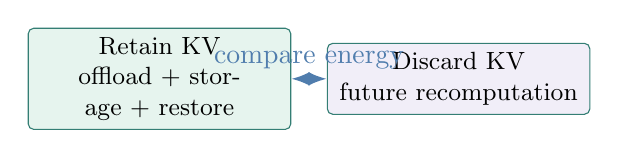
\begin{tikzpicture}[>=Latex,node distance=.45cm,box/.style={draw=Accent,rounded corners=2pt,fill=SoftMint,text width=3.1cm,minimum height=.72cm,align=center,font=\small}]
\node[box](a){Retain KV\\offload + storage + restore};\node[box,right=of a,fill=SoftLilac](b){Discard KV\\future recomputation};\draw[<->,thick,AccentBlue](a)--(b) node[midway,above]{compare energy};
\end{tikzpicture}\end{center}
\centering Potentially energy-efficient if $E_{retain}<E_{discard}$.\\[.18cm]\small Assumptions: one possible future reuse; $p$ is reuse probability. Shared batch energy, overlapping work, opportunity cost, and physical idle power need additional modeling. Allocated retention cost is not necessarily avoidable idle energy.
\src{Proposed analytical model: not an evaluated result.}\back{main-decision}{Decision path}\back{main-plan}{Research plan}
\end{frame}

\begin{frame}[t]{Backup B17 — Energy and Carbon Accounting Boundaries}
\target{backup-accounting}\tagline{Keep energy, carbon, and lifecycle allocation boundaries explicit}
\begin{columns}[T,onlytextwidth]\begin{column}{.49\textwidth}\begin{block}{Operational energy / carbon}\small GPU board, CPU, host DRAM, SSD, transfers, server baseline, shared batches, and overlapping prefetch / I/O.\\[.12cm]$E_{IT}=\int P_{IT}(t)dt$\\$C_{op}=\sum_t E_{IT,t}\,PUE_t\,CI_t$\end{block}\end{column}\begin{column}{.49\textwidth}\begin{block}{Embodied carbon / safeguards}\small Allocate lifecycle emissions over a declared service boundary.\\Avoid GPU/HBM double count; count shared batch work once; apply PUE once.\\Cache eviction does not undo manufacturing emissions. Lower occupancy need not lower physical idle draw.\\At fixed CI and PUE, energy and operational carbon rank configurations identically.\end{block}\end{column}\end{columns}
\src{Proposed accounting method informed by GreenCache, Sections 2.3 and 3.2.}\back{main-priorwork}{Prior work}\back{main-energy}{System model}
\end{frame}

\end{document}
